\chapter{O Participa.br}

O Participa.br - Plataforma Federal da Participação Social é um espaço colaborativo  	para participação social, escuta das demandas do povo e um espaço de dialogo da sociedade com o governo.

%

Ele tem como um dos seus principais objetivos, a criação de um canal de comunicação e participação entre cidadãos e gestores públicos. O Participa.br é uma ação do Gabinete Digital, que é uma iniciativa online do Governo Federal para ampliar o acesso do cidadão à informação pública, serviços, prestação de contas e participação popular nas decisões [1]. O Gabinete Digital foi anunciado pela presidenta Dilma Rousseff como resposta às manifestações ocorridas em todo território brasileiro em junho do ano de 2013, e uma de suas principais funções é realizar uma comunicação direta com a sociedade através das redes sociais.

%

No Participa.br, o cidadão pode se juntar a comunidades com temáticas do seu interesse, como por exemplo, educação, saúde, inclusão digital, entre outras. O Participa.br, permite também que participante crie uma comunidade com o tema de seu interesse, caso não exista. Isso é importante para que os usuários possam utilizar a ferramenta para debater temas que lhe interessem, isto torna a ferramenta mais atrativa. Para isso basta apenas que o usuário crie uma comunidade e alguém que administre ou modere a criação de comunidades na ferramenta do Participa.br aprove a mesma.

%

Uma das características do Participa.br é servir, além de um espaço de consulta pública, também como uma ferramenta para formulação de novas políticas públicas, como por exemplo, onde quem acessava a página inicial Participa.br durante os dias 19 de março de 2014 a 17 de abril de 2014, participava de um questionário para definir sobre a definição direitos e princípios fundamentais para garantir o futuro democrático e orientar a governança na internet. O participante tem direito a responder 3 perguntas, cada uma com um par de propostas, sem limites de respostas. A cada pergunta o usuário votava na opção que se concordava mais, caso não houvesse nenhuma proposta que ele mais se identificasse ele poderia sugerir novas propostas. O resultado dessa consulta foi enviado como uma Carta Proposta para o Comitê Gestor da Internet, o qual era o gestor do Arena NET Mundial, um evento realizado durante os dias 22, 23 e 24 de abril de 2014 na cidade de São Paulo, que tem como objetivo discutir ideias para garantir uma internet livre, colaborativa e democrática.

%

Quando o usuário acessa o Participa.br, ele só pode acessar as ferramentas de participação social se o mesmo se registrar na plataforma. O registro é bem simples, necessitando apenas alguns dados como nome de usuário, senha, nome, e-mail, entre outros. Após o registro, vai ser enviado um e-mail contendo o link para ativação do usuário (para evitar criação de spans de usuário). Após a ativação o cidadão já pode fazer comentários e contribuições na plataforma, personalizar o seu perfil, divulgar sua opinião em consultas públicas, manter o seu blog, participar e/ou criar comunidades, etc.

\section{Método de Desenvolvimento do Participa.br}

\section{Ferramentas de Participação Social}

De acordo com \cite{solagna2014metodologias} o desenho para um portal como o Participa.br não pode ser exaustivo, no sentido de oferecer todas as formas acabadas de participação digital, e sim instrumentalizar os atores sociais para que “instanciem” sua participação a partir do leque de possibilidades de influência nas políticas públicas e nas decisões do Estado, isto é, o podemos descrever o Participa.br como um framework de ferramentas de participação onde é possível acoplar novas ferramentas e metodologias de participação de acordo com a necessidade de cada gestor (conselhos, conferências, ouvidorias, etc.).

%

A imagem abaixo possui a atual arquitetura de funcionamento dos mecanismos de participação presentes no Participa.br. 

\graphicspath{{figuras/}}
\begin{figure}[H]
\centering
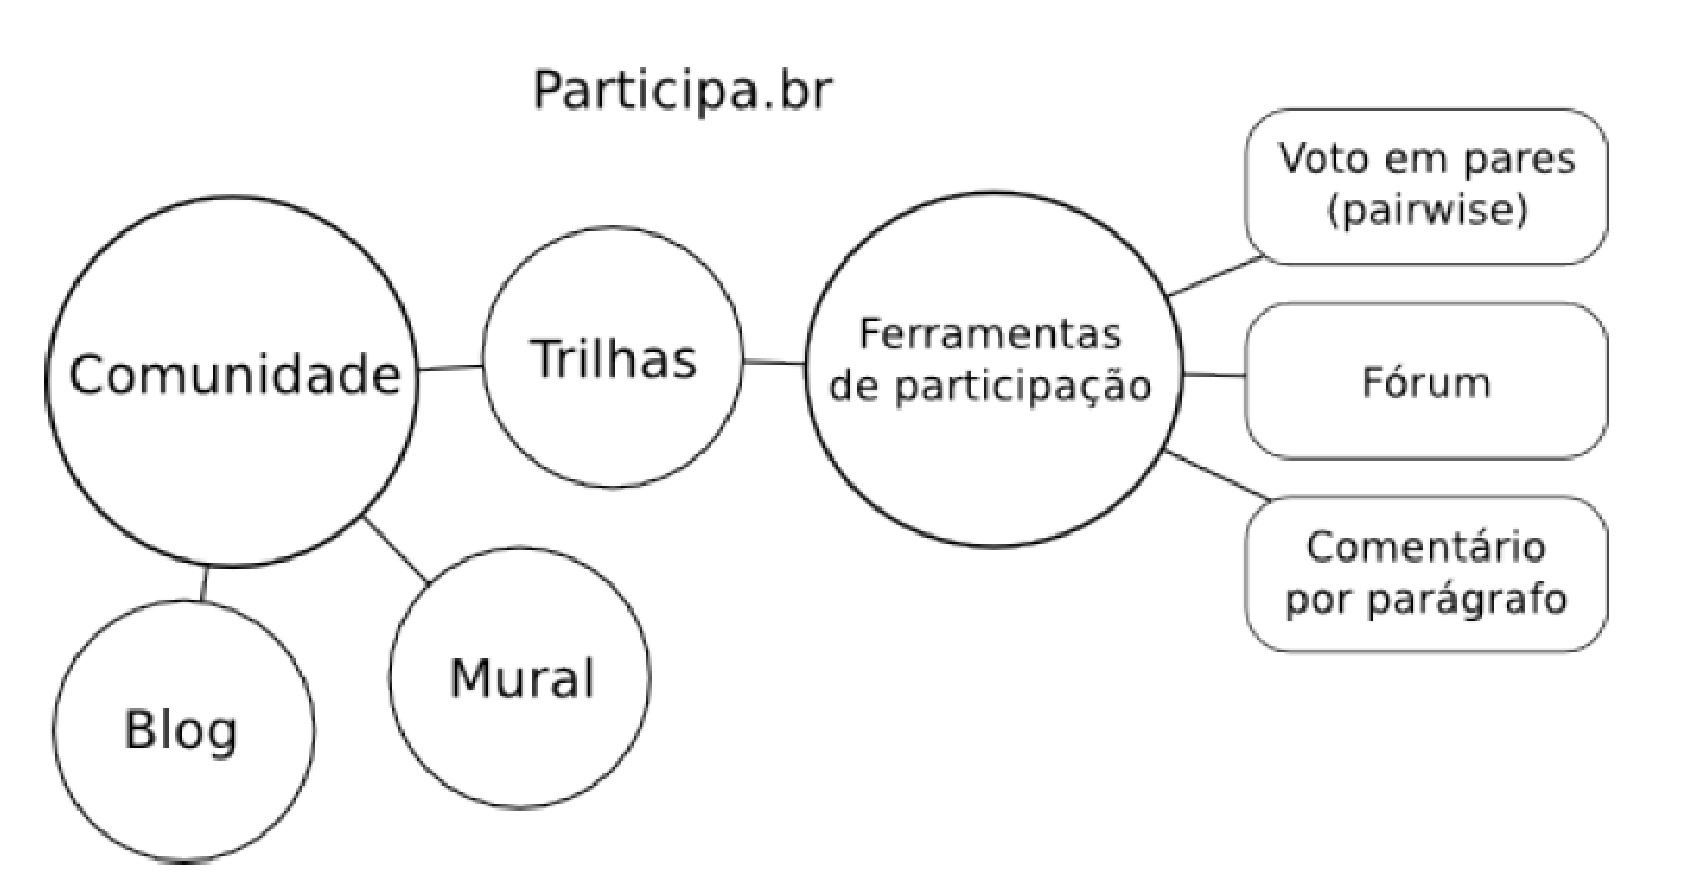
\includegraphics[width=0.7\textwidth]{arquitetura-ferramentas-participa}
\caption{Atual quadro de ferramentas de participação. Extraído de \cite{solagna2014metodologias}}
\label{fig:arquiteturaparticipa}
\end{figure}
















